\section{Introduction}
%

% training of NNs is hard
%
The success of Neural Networks (NN) is surprising, considering the hard optimization problem to 
be solved during training of NNs. Specifically, NN training is NP-complete~\citep{blumTraining3NodeNeural1988}, 
the loss surface and optimization problem are non-convex~\citep{dauphinIdentifyingAttackingSaddle2014,goodfellowQualitativelyCharacterizingNeural2015, lecunDeepLearning2015} and the parameter space to fit during training is high dimensional~\citep{brownLanguageModelsAre2020}. 
% Additionally, NN training is non-deterministic given its random initialization and sensitivity to
% hyperparameter selection~\citep{haninHowStartTraining2018,liVisualizingLossLandscape2018}. 
Additionally, NN training is sensitive to random initialization  and hyperparameter selection~\citep{haninHowStartTraining2018,liVisualizingLossLandscape2018}.
%
% non-convex -> multiple models
%
Together, this leads to an interesting characteristic of NN training: given a dataset and an architecture, different random initializations or hyperparameters lead to different minima on the loss surface and therefore result in different model parameters (i.e., weights and biases). Consequently, multiple training results in different NN models.
%
The resulting population of NN (referred to as \textit{model zoo})
is an interesting object to study: Do individual models of the model zoo have something in common? 
Do they form structures in weight space?
% How/what are the structures looking like?
What can we infer from such structures?
Can we learn representations of them?
Lastly, can such structures be exploited to generate new models with controllable properties?
\looseness-1

% Can a lower-dimensional manifold be learned representing these structures?
% Maybe, we can discover latent representations from such populations or even exploit them to sample unseen NN models?

% Do NN models evolve on unique, smooth trajectories in weight space during training? Can we predict model properties from the weights? Can we learn a latent representation of weights to enable model sampling? Can learning from model zoos facilitate new approaches for knowledge distillation and transfer learning?
%
% our hypothesis: populations are suuu-do-I-have-enough-uuuuper interesting
%
% Our hypothesis is that NN models evolve on unique, smooth trajectories in weight space during training. Consequently, such a population of NN models would form topological structures in weight space. We think that geometry, curvature and smoothness of the topology contains rich information about individual models, which can only be discovered from such populations.$
% update:

These questions have been partially answered in prior work.
Theoretical and empirical work demonstrates increasingly well-behaved loss surfaces for growing number of parameters \citep{goodfellowQualitativelyCharacterizingNeural2015,dauphinMetaInitInitializingLearning2019,liVisualizingLossLandscape2018}. The shape of the loss surface and the starting point is determined by hyperparameters and the initialization, respectively~\citep{liVisualizingLossLandscape2018}. NN training navigates the loss surface with iterative, gradient-based update schemes smoothed by momentum. The step length along a trajectory as well as the curvature are determined by the change of the loss as well as how aligned the subsequent updates are \citep{cazenavetteDatasetDistillationMatching2022,schurholtInvestigationWeightSpace2021}. Together, these findings suggest that populations of NN models evolve on unique and smooth trajectories in weight space.
Related work has empirically confirmed the existence of such structures in NNs~\citep{denilPredictingParametersDeep2013}, demonstrated the feasibility to learn representations of them, showed that they encode information on model properties ~\citep{unterthinerPredictingNeuralNetwork2020,eilertsenClassifyingClassifierDissecting2020,schurholtSelfSupervisedRepresentationLearning2021} and can be used to generate unseen models with desirable properties~\citep{schurholtHyperRepresentationsPreTrainingTransfer2022,schurholtHyperRepresentationsGenerativeModels2022,zhmoginovHyperTransformerModelGeneration2022,knyazevParameterPredictionUnseen2021}
%This leads us to the hypothesis, that NN models evolve on unique, smooth trajectories in weight space during training. Consequently, a population of NN models would form topological structures in weight space. Further, the curvature and smoothness of the topology may contain rich information about individual models, which can only be discovered from such populations.\looseness-1
%
%  - discriminative case
%  model property predictions
%
%
% With the proposed model zoos we would like to provide a foundation for systematic exploration of such properties.\looseness-1
To thoroughly answer the questions above, a large and systematically created dataset of model weights is necessary. 

\begin{figure*}[t]
\begin{minipage}[t]{1.0\textwidth}
\begin{center}
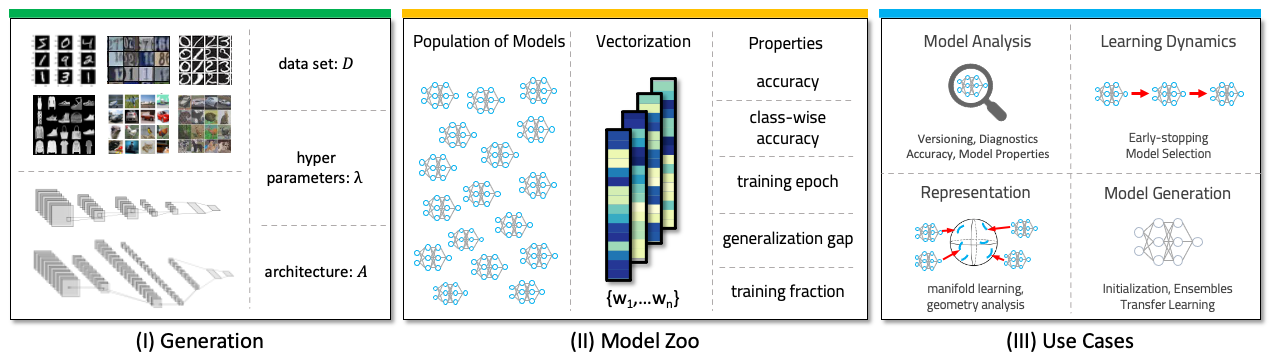
\includegraphics[trim=0in 0in 0in 0in, clip, width=1.0\linewidth]{imgs/model_zoo_overview_v2.png}
\vskip -0.1in
\caption{\small The proposed dataset of model zoos is trained on several image dataset with two CNN architectures and a multiple configurations of hyperparameters. The resulting population of neural network models is vectorized and made available with all meta-data such as the generating factors of the model zoo as well as the model properties such as accuracy, generalization gap and other. Potential use cases are (a) model property prediction, (b) inference of learning dynamics, (c) representation learning, or (d) model generation.
}
% \vskip -0.75cm
\label{fig:overview}    
\end{center}
\end{minipage}
\end{figure*}


%%%%%%%%%
%
% Problem: no standard dataset
%
Unfortunately, so far only few model zoos with specific properties have been published~\citep{unterthinerPredictingNeuralNetwork2020,eilertsenClassifyingClassifierDissecting2020, suchAtariModelZoo2019, schurholtSelfSupervisedRepresentationLearning2021}. While many machine learning domains have standardized datasets, there is no model zoo nor a benchmark to evaluate and compare against.
%
The lack of a standardized model zoos has three significant disadvantages: 
% existing ones are bad
(i), existing model zoos are usually designed for a specific purpose and of limited general utility. Their design space is rather sparse, covering only small portions of all available hyperparameter combinations. 
% small selection of models only.
Moreover, some existing zoos are generated on synthetic tasks and are small, containing only a small population of models; 
% transaction cost of generating new datasets
(ii), researchers have to choose between using an existing zoo or generating a new one for each new experiment, weighing disadvantages of existing zoos against the effort and computational resources required to generate a new zoo; 
% not comparable
(iii), a new model zoo causes subsequent work to lose comparability to existing research. Therefore, the lack of a benchmark model zoo significantly increases the friction for new research.


%%%%%%%%%%
%
% Solution: Standard dataset is needed
%
\textbf{Our contributions:}
To study the behaviour of populations of NNs, we publish a large-scale model zoo of diverse populations of neural network models with controlled generating factors of model training.  
Special care has been taken in their design and the used protocols for training. To do so, we have defined and restricted the generating factors of model zoo training to achieve desired zoo 
characteristics.\looseness-1

%
% mode details about the model zoos
%
The zoos are trained on eight standard image classification datasets, with a broad range of hyperparameters and contain thousands of configurations. Further, we add sparsified \textit{model zoo twins} to each of these zoos.
%For six of the image datasets, we create three zoos with different modes of variations to control the type of variation in the properties of the zoo.  
%
All together, the zoos include a total of 50'360 unique image classification NNs, resulting in over 3’844’360 collected model states.


%
% use-cases ->>> the fourth use case is missing
%
Potential use-cases for the model zoo include (a) model analysis for reliability, bias, fairness, or adversarial vulnerability, (b) inference of learning dynamics for efficiency gain, model selection or early stopping, (c) representation learning of such populations, or (d) model generation.
%Potential use-cases of the model zoos are (i) the analysis of NNs for reliability, bias, fairness, or adversarial vulnerability, (ii) a similarity measure between neural network models, which can be used for versioning of models or intellectual property protection, (iii) understanding of learning dynamics to save computational cost during training.
%Insights gained from the investigation of such model zoos could be used in the analysis of models, lead to better understanding of learning dynamics and be incorporated in the generation of new models.
%
% benchmark
%
Additionally, we present an analysis of the model zoos and a set of experimental setups for benchmarks on these use-cases and initial results as foundation for evaluation and comparison.



%
% closing statement
%
With this work we provide a standardized dataset of diverse model zoos connected to popular image datasets, its corresponding meta-data and performance evaluations to the machine learning research community. All data is made publicly available to foster community building around the topic and to provide a ground for use beyond the defined benchmark tasks. 
%
An overview of the proposed dataset and benchmark as well as potential use-cases can be found in Fig.~\ref{fig:overview}



